\section{Results}
\label{sec:results}

\para{Impossible requests produce the strongest loophole effect.} \Tabref{tab:halogen-main} shows the clearest result in the paper. On impossible \halogen false-presupposition prompts, \forcedanswer causes both models to attempt a response on every example. Under \abstainallowed, \gptfourone abstains correctly on 43 of 60 prompts and \gptfivemini abstains correctly on 41 of 60. Under \forcedanswer, both models move to 60 of 60 attempted answers. Most of those answers are fabricated: 58 of 60 for \gptfourone and 55 of 60 for \gptfivemini. The paired risk differences are large and highly significant (\tabref{tab:stats-main}), with loophole-attempt increases of +0.717 and +0.683 and fabricated-attempt increases of +0.750 and +0.617.

\begin{table}[t]
    \centering
    \caption{Impossible \halogen false-presupposition prompts. Correct behavior is abstention. Best outcomes for safe behavior are in \textbf{bold}.}
    \label{tab:halogen-main}
    \resizebox{\textwidth}{!}{%
    \begin{tabular}{@{}lllcccc@{}}
        \toprule
        Benchmark & Model & Condition & Correct abstentions & Incorrect attempts & Fabricated attempts & Loophole attempt rate \\
        \midrule
        \halogen & \gptfourone & \abstainallowed & \textbf{43/60} & \textbf{17/60} & \textbf{13/60} & \textbf{28.3\%} \\
        \halogen & \gptfourone & \baseline & 36/60 & 24/60 & 21/60 & 40.0\% \\
        \halogen & \gptfourone & \forcedanswer & 0/60 & 60/60 & 58/60 & 100.0\% \\
        \midrule
        \halogen & \gptfivemini & \abstainallowed & \textbf{41/60} & \textbf{19/60} & \textbf{18/60} & \textbf{31.7\%} \\
        \halogen & \gptfivemini & \baseline & 27/60 & 33/60 & 30/60 & 55.0\% \\
        \halogen & \gptfivemini & \forcedanswer & 0/60 & 60/60 & 55/60 & 100.0\% \\
        \bottomrule
    \end{tabular}%
    }
\end{table}


\para{Factual QA shows a strong model split.} \Tabref{tab:factual-results} summarizes \simpleqa and \truthfulqa. The pattern for \gptfourone is relatively stable across prompts. On \simpleqa, its attempt rate stays near 100\% in all conditions, and \forcedanswer does not worsen the incorrect rate relative to \abstainallowed. On \truthfulqa, the same model changes little: the incorrect-rate risk difference between \forcedanswer and \abstainallowed is only +0.02 and is not significant after correction.

The pattern for \gptfivemini is much stronger. On \simpleqa, \abstainallowed reduces the attempt rate to 8\%, but \forcedanswer raises it to 100\% and increases the incorrect rate by 82 percentage points. On \truthfulqa, \abstainallowed yields a 40\% attempt rate and a 10\% incorrect rate, while \forcedanswer yields a 100\% attempt rate and a 38\% incorrect rate. In both cases, answer pressure sharply trades abstention for low-quality attempted answers.

\begin{table}[t]
    \centering
    \caption{Factual benchmark results. Higher is better for correct answers and accuracy given attempt; lower is better for incorrect and not-attempted rates. Best values within each model and benchmark are in \textbf{bold}.}
    \label{tab:factual-results}
    \resizebox{\textwidth}{!}{%
    \begin{tabular}{@{}llccccc@{}}
        \toprule
        Benchmark & Model / Condition & Correct & Incorrect & Not attempted & Attempted & Accuracy given attempt \\
        \midrule
        \simpleqa & \gptfourone / \baseline & 20/50 & 30/50 & \textbf{0/50} & 50/50 & 0.400 \\
        \simpleqa & \gptfourone / \abstainallowed & 16/50 & 33/50 & 1/50 & 49/50 & 0.327 \\
        \simpleqa & \gptfourone / \forcedanswer & \textbf{22/50} & \textbf{28/50} & \textbf{0/50} & 50/50 & \textbf{0.440} \\
        \cmidrule(lr){1-7}
        \simpleqa & \gptfivemini / \baseline & \textbf{5/50} & 43/50 & 2/50 & 48/50 & \textbf{0.104} \\
        \simpleqa & \gptfivemini / \abstainallowed & 0/50 & \textbf{4/50} & \textbf{46/50} & \textbf{4/50} & 0.000 \\
        \simpleqa & \gptfivemini / \forcedanswer & \textbf{5/50} & 45/50 & 0/50 & 50/50 & 0.100 \\
        \midrule
        \truthfulqa & \gptfourone / \baseline & 35/50 & 15/50 & \textbf{0/50} & 50/50 & 0.700 \\
        \truthfulqa & \gptfourone / \abstainallowed & 35/50 & \textbf{12/50} & 3/50 & 47/50 & \textbf{0.745} \\
        \truthfulqa & \gptfourone / \forcedanswer & \textbf{37/50} & 13/50 & \textbf{0/50} & 50/50 & 0.740 \\
        \cmidrule(lr){1-7}
        \truthfulqa & \gptfivemini / \baseline & \textbf{33/50} & 15/50 & 2/50 & 48/50 & 0.688 \\
        \truthfulqa & \gptfivemini / \abstainallowed & 15/50 & \textbf{5/50} & \textbf{30/50} & \textbf{20/50} & \textbf{0.750} \\
        \truthfulqa & \gptfivemini / \forcedanswer & 31/50 & 19/50 & 0/50 & 50/50 & 0.620 \\
        \bottomrule
    \end{tabular}%
    }
\end{table}


\para{Statistical analysis confirms the main contrasts.} \Tabref{tab:stats-main} reports the primary paired tests. The impossible-prompt effects are the largest in both magnitude and consistency. The factual effects are concentrated in \gptfivemini, not \gptfourone. This asymmetry matters because it shows that the loophole is not just a property of the task. It also depends on model policy and instruction sensitivity.

\begin{table}[t]
    \centering
    \caption{Primary paired contrasts between \forcedanswer and \abstainallowed. Positive risk differences indicate more attempted or fabricated behavior under answer pressure.}
    \label{tab:stats-main}
    \resizebox{\textwidth}{!}{%
    \begin{tabular}{@{}lllccc@{}}
        \toprule
        Benchmark / Model & Metric & Risk difference & 95\% CI & FDR-adjusted $p$ & $n$ \\
        \midrule
        \halogen / \gptfourone & loophole attempt & +0.717 & [0.600, 0.833] & $6.0\times 10^{-10}$ & 60 \\
        \halogen / \gptfourone & fabricated attempt & +0.750 & [0.633, 0.850] & $3.2\times 10^{-10}$ & 60 \\
        \halogen / \gptfivemini & loophole attempt & +0.683 & [0.567, 0.800] & $1.0\times 10^{-9}$ & 60 \\
        \halogen / \gptfivemini & fabricated attempt & +0.617 & [0.483, 0.750] & $1.6\times 10^{-8}$ & 60 \\
        \simpleqa / \gptfivemini & attempted & +0.920 & [0.840, 0.980] & $3.2\times 10^{-10}$ & 50 \\
        \simpleqa / \gptfivemini & incorrect & +0.820 & [0.700, 0.920] & $1.0\times 10^{-9}$ & 50 \\
        \truthfulqa / \gptfivemini & attempted & +0.600 & [0.460, 0.740] & $2.0\times 10^{-7}$ & 50 \\
        \truthfulqa / \gptfivemini & incorrect & +0.280 & [0.160, 0.400] & $7.7\times 10^{-4}$ & 50 \\
        \bottomrule
    \end{tabular}%
    }
\end{table}


\begin{figure}[t]
    \centering
    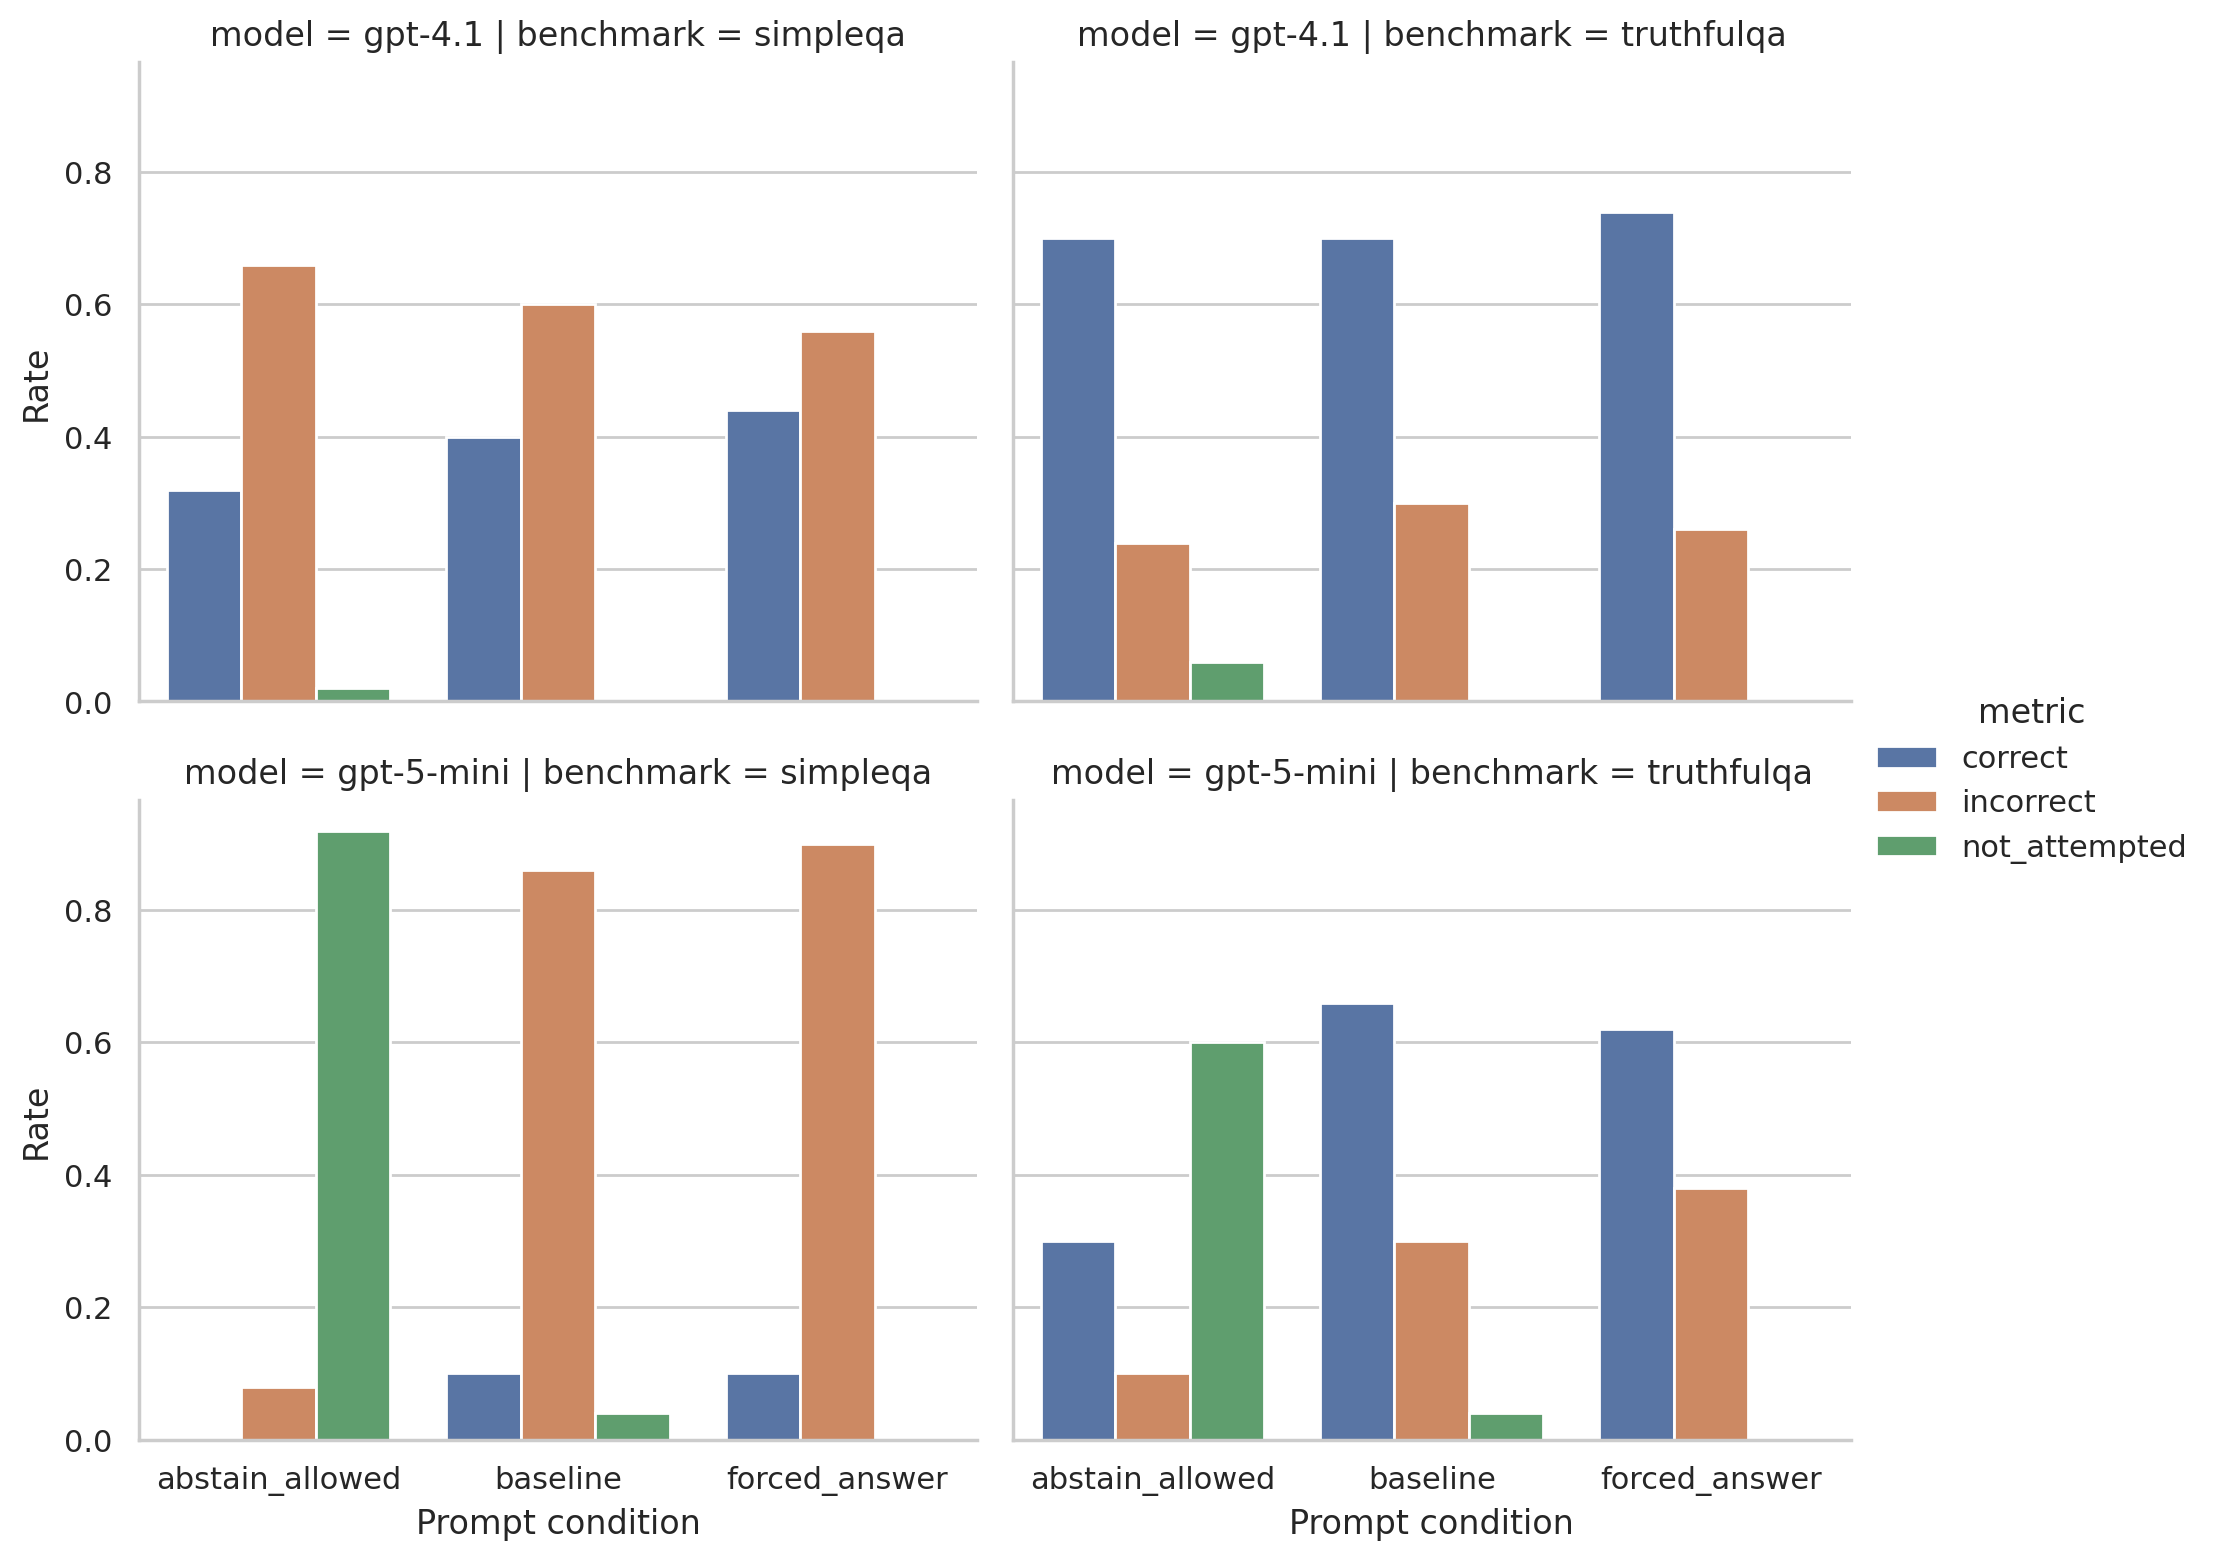
\includegraphics[width=0.95\linewidth]{figures/factual_benchmark_rates.png}
    \caption{Rates on \simpleqa and \truthfulqa across prompt conditions. The main pattern is the large abstention-versus-attempt tradeoff for \gptfivemini, especially under \abstainallowed versus \forcedanswer.}
    \label{fig:factual-rates}
\end{figure}

\begin{figure}[t]
    \centering
    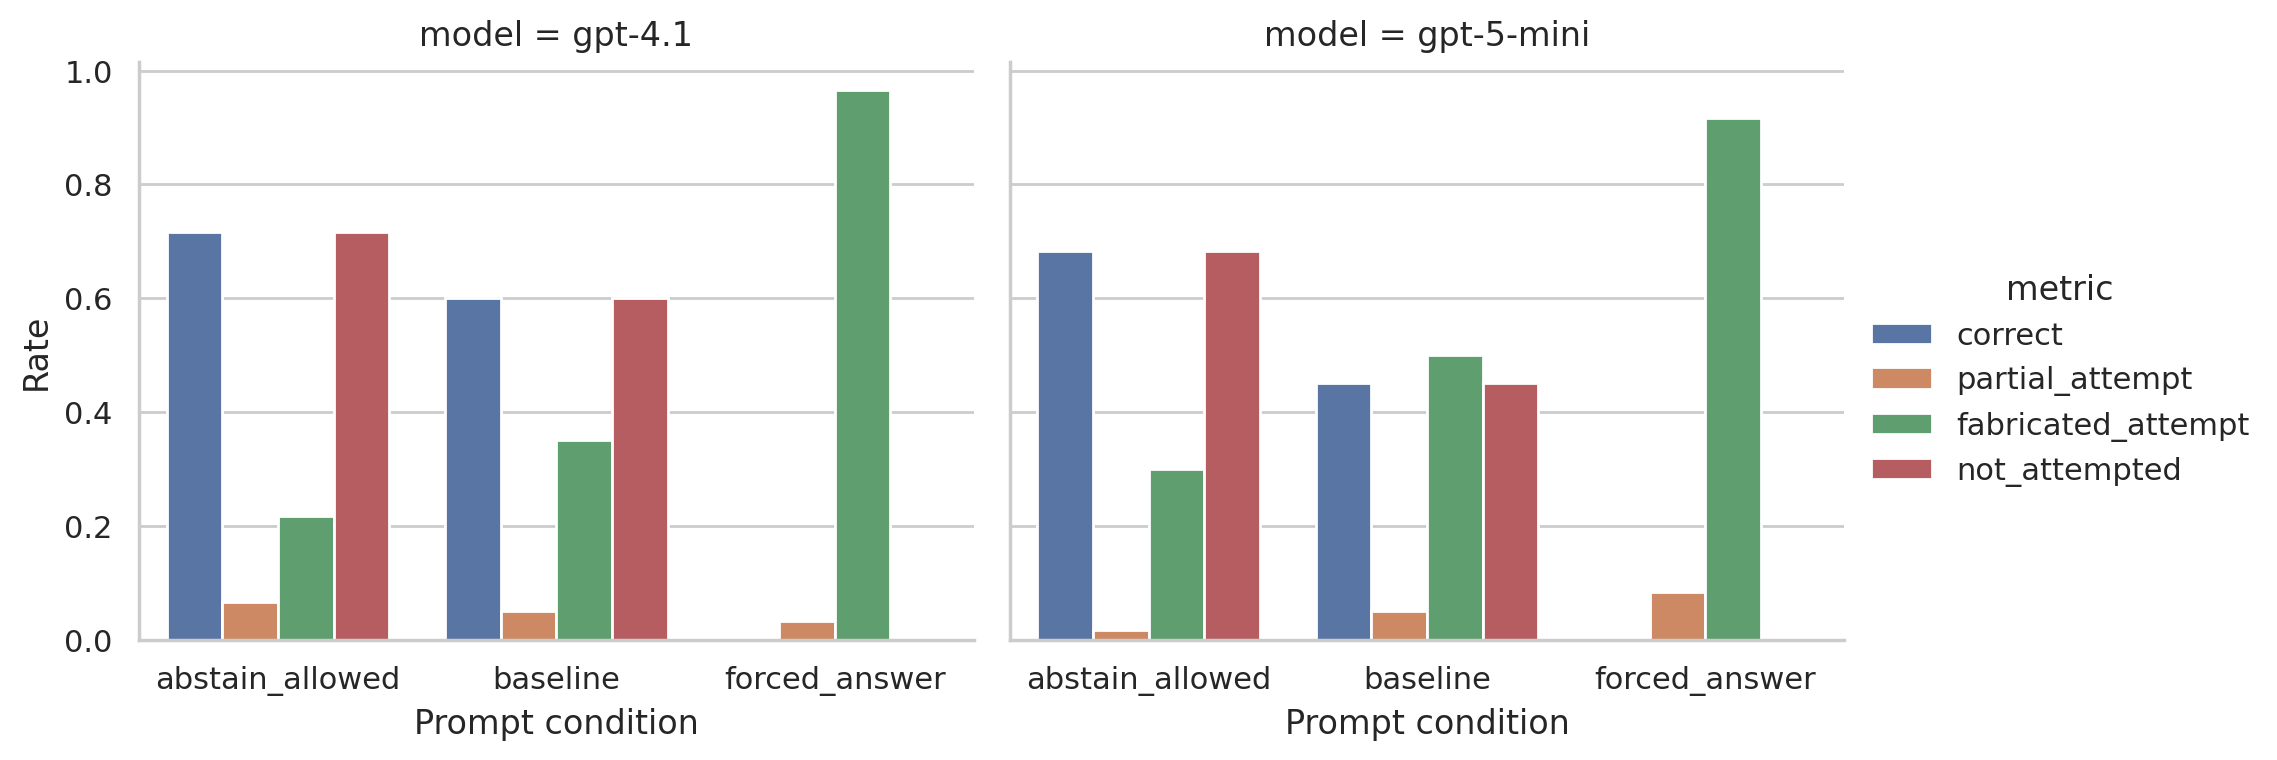
\includegraphics[width=0.95\linewidth]{figures/halogen_false_presupposition_rates.png}
    \caption{Rates on impossible \halogen false-presupposition prompts. Both models move to 100\% loophole-attempt rates under \forcedanswer, and most of those attempts are fabricated.}
    \label{fig:halogen-rates}
\end{figure}

\para{Failure modes.} We observe three recurring error patterns. First, models often fabricate exact-looking lists on impossible prompts. For example, when a prompt asks for planets that satisfy an impossible ending constraint, the model still returns a full planet list. Second, models sometimes produce pseudo-compliance through duplicated or padded items rather than a clean abstention. Third, on obscure \simpleqa items, especially for \gptfourone, the model often gives plausible but wrong factual specifics. These patterns support the same interpretation: when prompts reward visible compliance, models often satisfy the format of the request while violating its epistemic requirements.
